% ----------------------- TODO ---------------------------
% Diese Daten müssen pro Blatt angepasst werden:
\newcommand{\NUMBER}{1}
\newcommand{\EXERCISES}{5}
% Diese Daten müssen einmalig pro Vorlesung angepasst werden:
\newcommand{\COURSE}{HPC Lab - Assignment 4}

\newcommand{\STUDENTA}{Zirong Cai}
\newcommand{\STUDENTB}{Phuong Nguyen}
\title{\vspace{-2em} Assignment 4 - Profiler \vspace{-0.5em}}
\author{ \STUDENTA, \STUDENTB}
\date{\today {\vspace{-1cm}}}

% ----------------------- TODO ---------------------------

\documentclass[article]{scrartcl}

\usepackage[utf8]{inputenc}
\usepackage[ngerman]{babel}
\usepackage{amsmath}
\usepackage{amssymb}
\usepackage{fancyhdr}
\usepackage{color}
\usepackage{graphicx}
\usepackage{lastpage}
\usepackage{listings}
\usepackage{tikz}
\usepackage{pdflscape}
\usepackage{float}
\usepackage{polynom}
\usepackage{hyperref}
\usepackage{tabularx}
\usepackage{forloop}
\usepackage{geometry}
\usepackage{listings}
\usepackage{caption}
\usepackage{subcaption}
\usepackage{subcaption}
\usepackage{fancybox}
\usepackage{tikz}
\usepackage{algpseudocode,algorithm,algorithmicx}
%\usepackage{biblatex}
\usepackage{cite}

\setkomafont{title}{\normalsize}
\setkomafont{author}{\small}
\setkomafont{date}{\small}
\setkomafont{section}{\normalfont \normalsize \textbf}
\setkomafont{subsection}{\normalfont}
\renewcommand*{\thesubsection}{\alph{subsection}}

\setkomafont{subsubsection}{\normalfont\itshape}

\lstset { %
    language=C++,
    backgroundcolor=\color{black!5}, % set backgroundcolor
    basicstyle=\footnotesize,% basic font setting
}
%\captionsetup[lstlisting]{ format=listings, labelfont=white, textfont=white}

%Definiere Let-Command für algorithmen
%\newcommand*\Let[2]{\State #1 $\gets$ #2}

%\input kvmacros

%Größe der Ränder setzen
\geometry{a4paper,left=3cm, right=3cm, top=3cm, bottom=3cm}

%Kopf- und Fußzeile
\pagestyle {fancy}
\fancyhead[L]{\STUDENTA, \STUDENTB}
\fancyhead[R]{\COURSE}

\fancyfoot[L]{}
\fancyfoot[R]{Page \thepage /\pageref*{LastPage}}

\begin{document}


\maketitle
\thispagestyle{fancy}

\section{ Quicksort – Intel VTune Amplifier XE (2P)}
\subsection{Optimal final clause}
Using Basic Hotspots, the two important matrics we can get are Elapsed Time and CPU time which are defined as:
\begin{itemize}
    \item Elapsed Time: the wall clock time from start to end of the execution
    \item CPU time: the quantity of processor time taken by the processes.
\end{itemize}
As a end user, what we want is of course faster response time, and we don't care about CPU pressure. In this case, we want to get the sorted array as soon as possible, meaning lower elapsed time.\\
In the table \ref{tab::final}, we listed the elapsed time of our quicksort application with respect to different thread numbers and different final-clauses.
cond\{i\} correspond to:
$$CurrentArrayLength < DataSize / i, i = 2,4,8,14,28$$
We can see that the clauses that give us the lowest elapsed time are either under condition4 or condition5. We first assume that there's a best final clause between condition4 and condition5, we didn't find it because the granularity we use here is too large.
\begin{table}[h!]
    \centering
  \begin{tabular}{ |p{3cm}|p{1cm}|p{1cm}|p{1cm}|p{1cm}|p{1cm}|  }
    \hline
    NUM\_THREAD & cond2 & cond4 & cond8 & cond14 & cond28\\
     \hline
     2&0.791&0.920&0.670&\textbf{0.658}&0.876\\
     \hline
     4 & 0.583&0.600&0.511&0.916&\textbf{0.489}\\
    \hline
    8 &0.791&0.503&0.679&0.656&\textbf{0.436}\\
    \hline
    14 & 0.638&0.752&0.648&0.661&\textbf{0.547}\\
   \hline
   28 &0.694&1.043&0.954&\textbf{0.677}&0.901\\
    \hline
    \end{tabular}
    \caption{Elapsed Time With Different final-clauses Using Datasize=2000000}
    \label{tab::final}
\end{table}

So we reduce the granularity to 1 and examine all possibilities. And we find that for different thread numbers, the final clause 
$$CurrentArrayLength < 75000(\approx DataSize / 26)$$
gives us the best performance.
\subsection{Other Analysis types}
\begin{itemize}
    \item performance-snapshot: useful to get a quick snapshot of our application performance and identify next
    steps for deeper analysis.
    \item memory-consumption: Analyze memory consumption by our application, its distinct memory
    objects and their allocation stacks. Since our application is compute bound but not memory bound, this feature is not useful for us.
    \item microarchitecture: Analyze CPU microarchitecture bottlenecks affecting the performance of
    our application. Since our code only uses some compare and exchange operations, this is also not useful for our application.
    \item threading: Discover how well our application is using parallelism to take advantage
    of all available CPU cores. This could be useful for us to find the best final clause.
    \item io: Analyze utilization of IO subsystems, CPU, and processor buses. Not useful since our application don't have much IO.
\end{itemize}

\subsection{Does the optimal final clause depend on the number of threads or the array length?}
As discussed above, the optimal final clause dose not depend on the number of threads.\\
To find out whether the optimal final clause depend on the array length or not, we fixed the number of threads to 14 and profile our allication with different data size, 
we then get the table \ref{tab::final_datasize} which gives us a similar result that the optimal final clause is around 26, not exactly 26, but near by 26, so we may conclude that 
the optimal final clause does also not depend on the data size.
\begin{table}[h!]
    \centering
  \begin{tabular}{ |p{2cm}|p{1cm}|p{1cm}|p{1cm}|p{1cm}|p{1cm}|p{1cm}|p{1cm}|p{1cm}|p{1cm}|p{1cm}|  }
    \hline
    Data Size & cond2 & cond4 & cond8 & cond14 & cond16 & cond20&cond22&cond24&cond26&cond28\\
     \hline
     5000000&5.884&3.382&0.598&17.064&3.510&3.866&4.742&4.356&3.566&\textbf{0.538}\\
     \hline
     10000000 & 1.545&1.261&0.915&7.590&2.669&3.355&8.594&\textbf{0.833}&3.651&10.860\\
    \hline
    \end{tabular}
    \caption{Elapsed Time With Different Final-clauses Under Different Data Size}
    \label{tab::final_datasize}
\end{table}

\subsection{Question}
\begin{figure}[htpb]
    \centering
    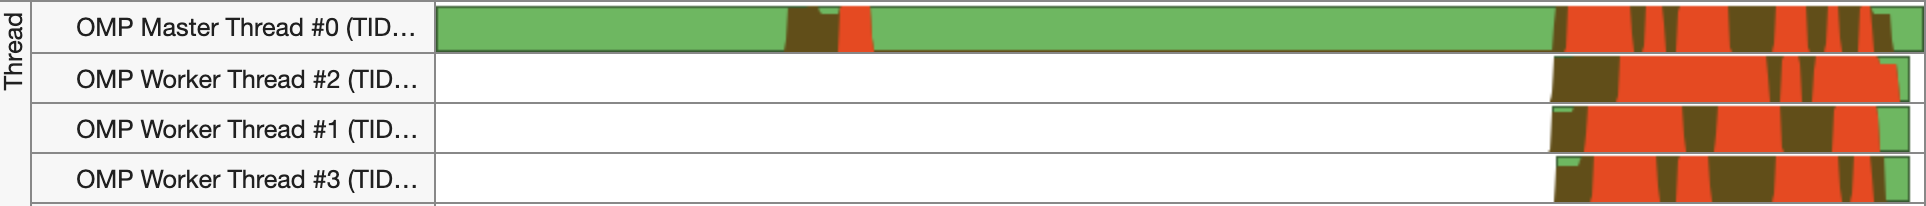
\includegraphics[width=\textwidth,keepaspectratio=true]{../figs/bottomup1.png}
    \caption{BottomUp with 8 threads and cond14 under Data Size=2000000}
    \label{fig:quickQes}
\end{figure}
\begin{figure}[htpb]
    \centering
    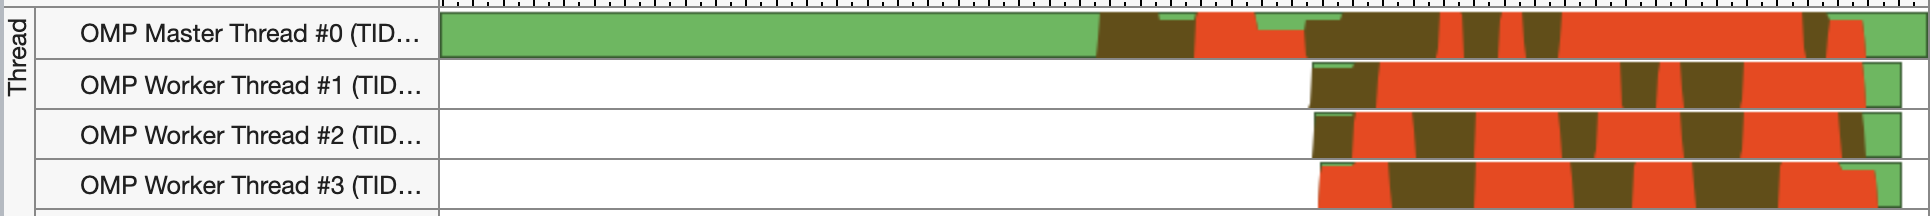
\includegraphics[width=\textwidth,keepaspectratio=true]{../figs/bottomup2.png}
    \caption{BottomUp with 8 threads and cond8 under Data Size=2000000}
    \label{fig:quickQes2}
\end{figure}
In figure \ref{fig:quickQes}, we saw that after the initialization of the data array, thread 0 start to execute the code of quicksort, but then the process stays idle for a quite long time,
while under other conditions, e.g. in figure \ref{fig:quickQes2} there's no such idle time. I am quite confused since there are no I/O or barrier(well there does exist a task wait barrier but as far as i know, task wait won't block a thread) after the first execution.

\section{CG – Scalasca (3P)}
\subsection{Automatic instrumentation}
We profiled the CG implementation with 28 MPI processes, the output data was visualized with Cube and presented in Figure \ref{fig:sca_compload}. The program spent 1274 second in the main computation which is 94.1\% of the total runtime. As we can see in the third column, each rank spent roughly 45 seconds. This result looks pretty good in term of load balancing. From this figure, we also saw that the program took 1354 seconds in total but only 6.09 seconds for Computational Load Imbalance, which is 0.5\% only. Figure \ref{fig:sca_loadim} shows the detail of load imbalance in each rank. We can see that some ranks are overloaded while some other are underloaded, but the difference is not significant. 
\begin{figure}[htpb]
    \centering
    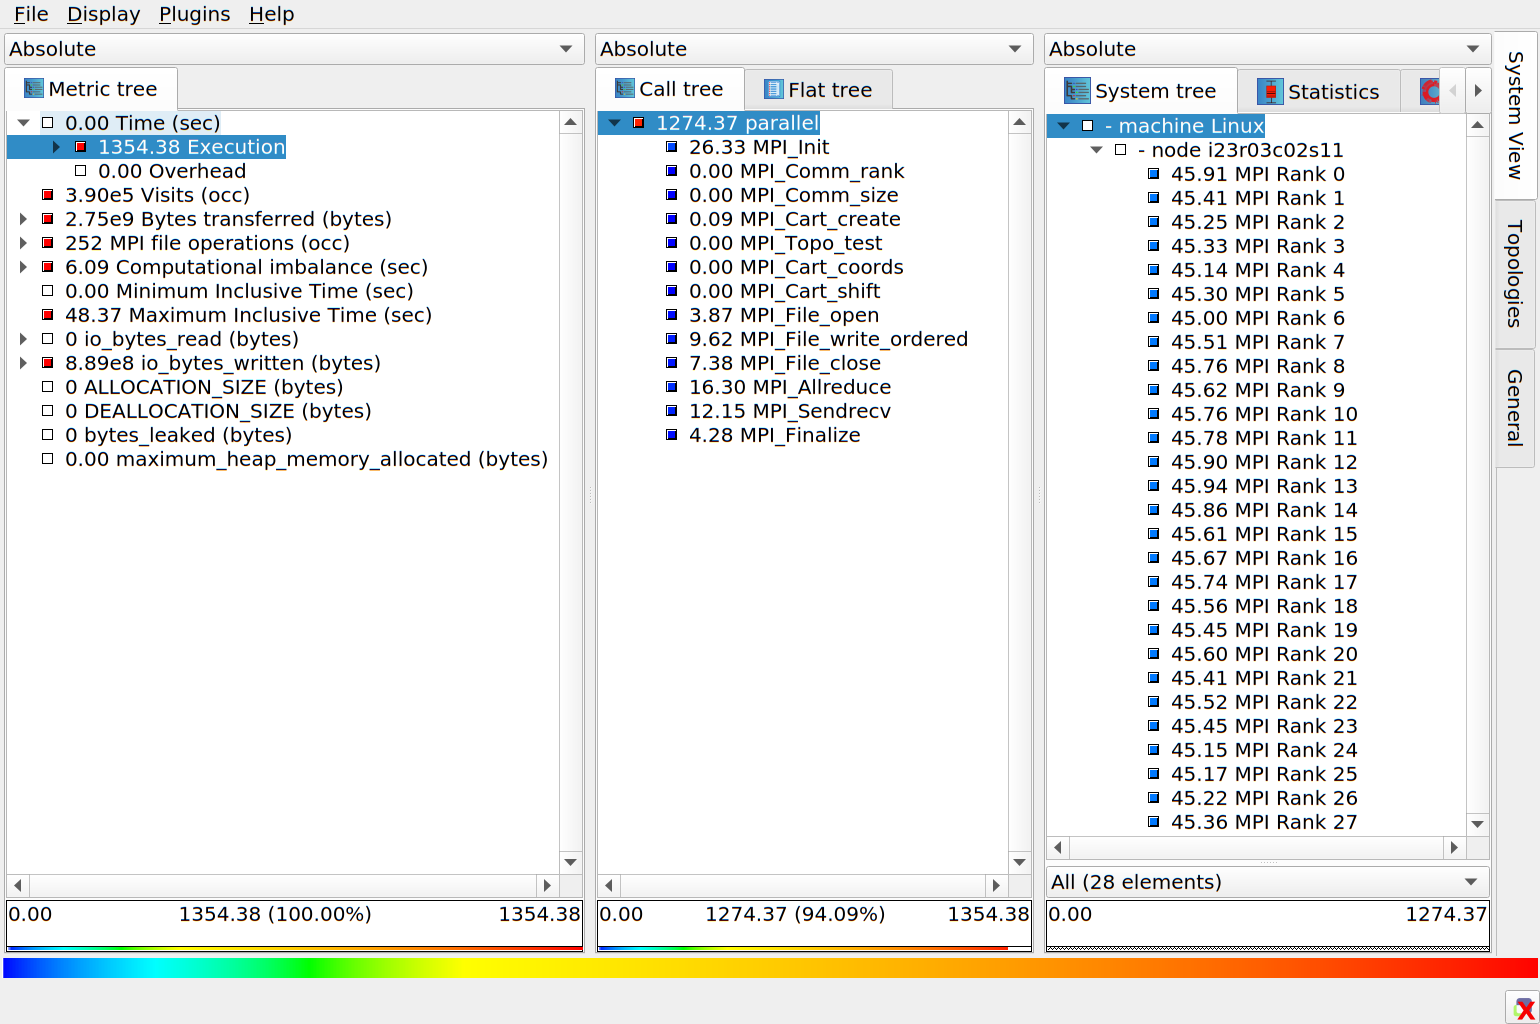
\includegraphics[width=.9\textwidth,keepaspectratio=true]{../figs/3_1_Cube_Computation.png}
    \caption{Profiling of CG, Computation Load}
    \label{fig:sca_compload}
\end{figure}
\begin{figure}[htpb]
    \centering
    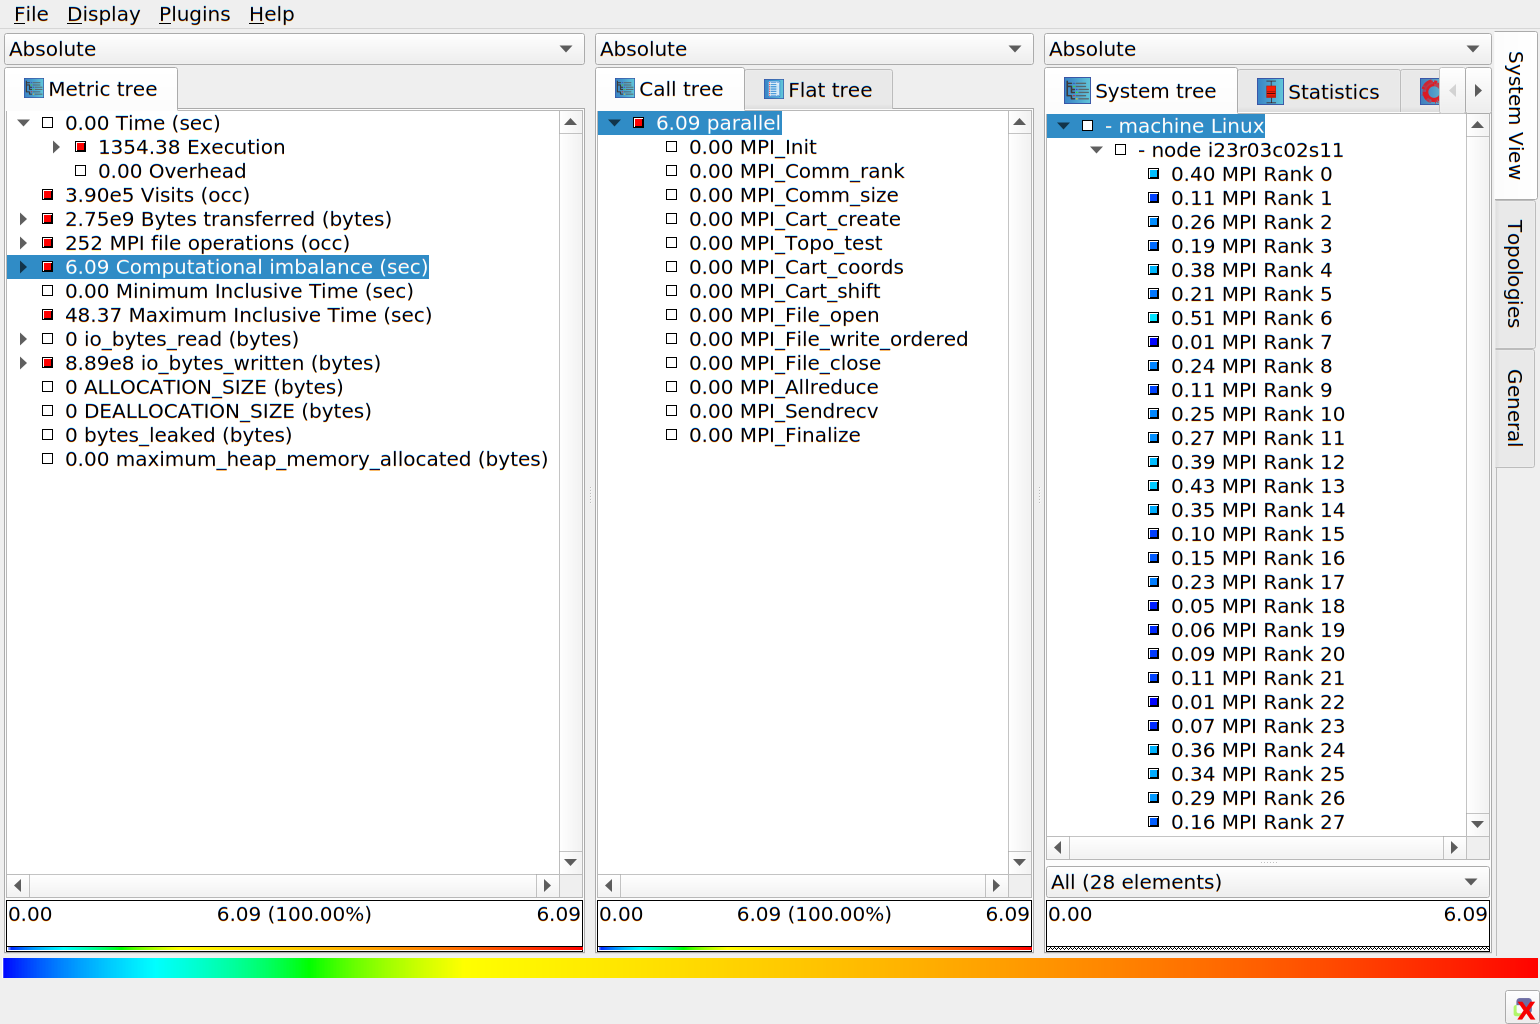
\includegraphics[width=.9\textwidth,keepaspectratio=true]{../figs/3_1_Cube_LoadImbalance.png}
    \caption{Profiling of CG, Load Imbalance}
    \label{fig:sca_loadim}
\end{figure}


\subsection{Manual instrumentation}
For manual instrumentation, we decided to profile the \textit{solver} function only since it's the heart of the program. We did it by defining a profiling region inside the function as describe below:
\begin{lstlisting}[frame=single]
void solve(struct_param *param, std::size_t cg_max_iterations, double cg_eps)    
{                                                                                                     
  SCOREP_USER_REGION_DEFINE( handle )                                          
  SCOREP_USER_REGION_BEGIN( handle, "solve", SCOREP_USER_REGION_TYPE_FUNCTION) 

    // Do the actual computation
    ...

  SCOREP_USER_REGION_END( handle)
}
\end{lstlisting}
The profiling output is presented in the Figure \ref{fig:sca_function}.
\begin{figure}[htpb]
    \centering
    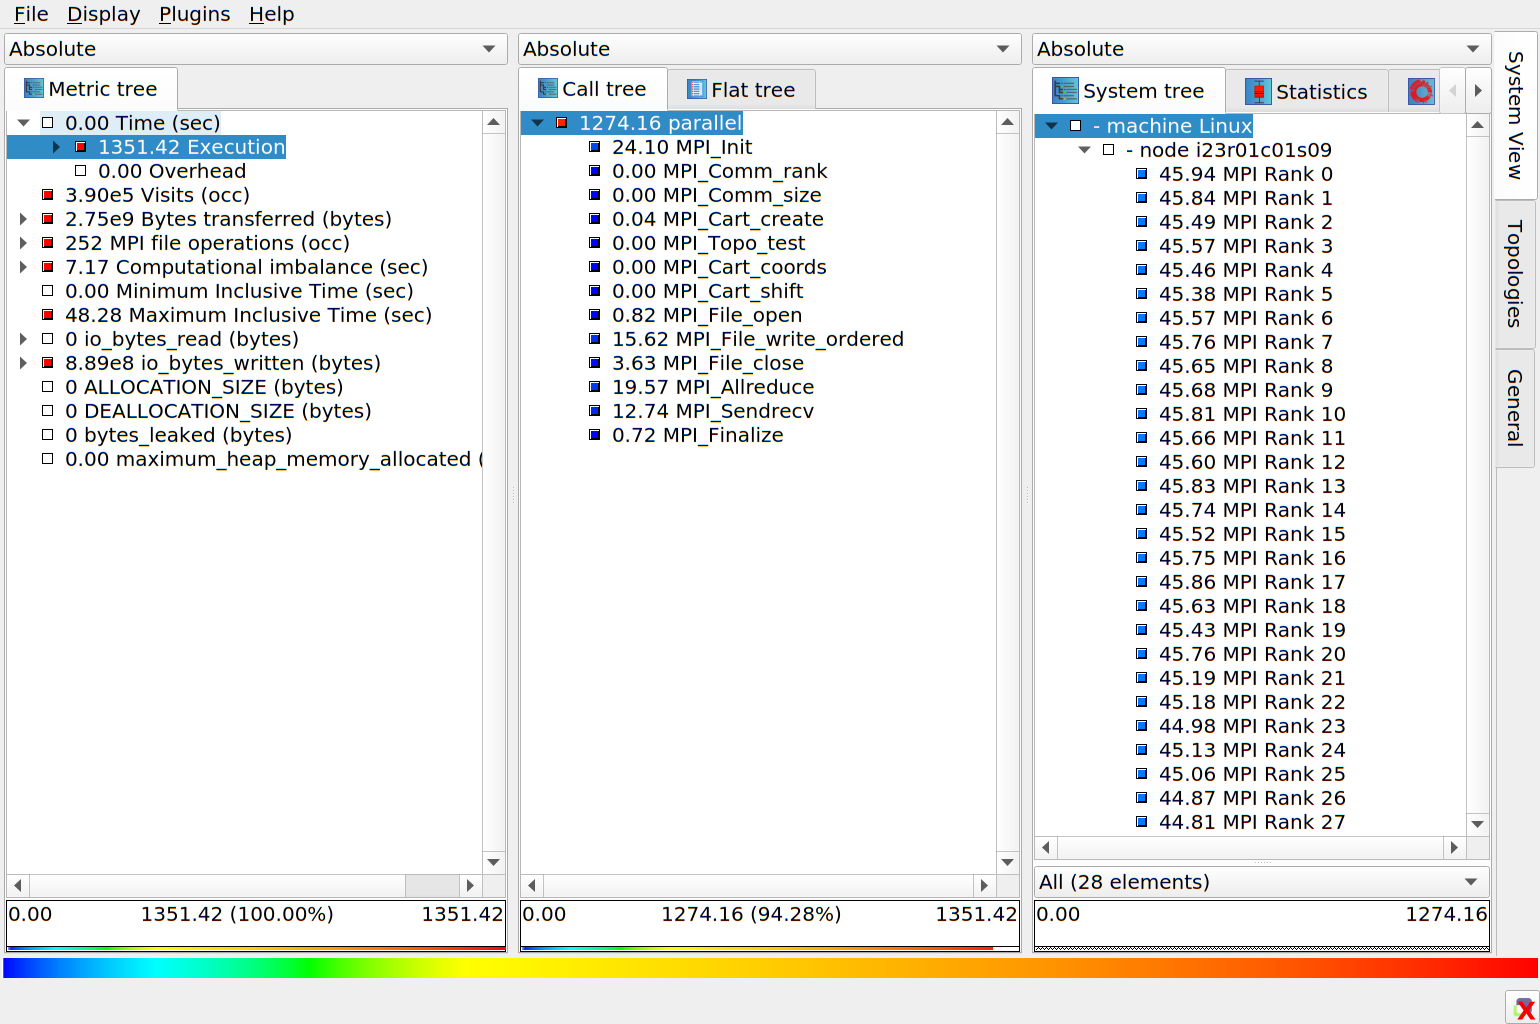
\includegraphics[width=.9\textwidth,keepaspectratio=true]{../figs/3_2_Cube_Function.png}
    \caption{Manual profiling of solve function}
    \label{fig:sca_function}
\end{figure}
Compares to the previous profile output, there is no big difference. However, one can notice that the computational imbalance time is different, so is the total runtime. There is no much different since the program spent most of the time in this solver function, rather then others.

\subsection{Hybrid Implementation of CG}
\paragraph{Implementation}
We implemented OpenMP \textit{parallel for} for loops in following functions: \textit{g\_copy}, \textit{g\_dot\_product}, \textit{g\_scale}, \textit{g\_scale\_add}, \textit{g\_product\_operator}. Besides, to optimize for NUMA, we also implemented "First-touch" which is parallelizing the data initialization in \textit{init\_grid}, \textit{init\_b}, \textit{g\_copy}.
In addition to the MPI code from the last worksheet, we have successfully implemented MPI File I/O for parallelized outputing. 
\paragraph{Performance}
We tested out hybrid implementation with different configuration and number of threads per MPI. The best results are given when the number of OpenMP threads equal to 7, and the bind set are:
\begin{verbatim}
KMP_AFFINITY=granularity=core,compact,1,0
I_MPI_PIN_DOMAIN=omp 
I_MPI_PIN_ORDER=compact
I_MPI_PIN_CELL=core
\end{verbatim}
This seems reasonable since on our system each NUMA node has 7 cores. With this configuration, each MPI process has 7 threads in the team, binds to 7 cores in the same NUMA node which is good for data accessing. \\
The performance of this hybrid implemented is presented in the Figure \ref{fig:compare_hybrid}, in comparison with the performance of pure MPI implementation. The performance of Hybrid approach is the similar to the pureMPI, even for the test on 4 nodes or 8 nodes. We would expect the Hybrid one has better performance since it can ultilize both advantages of shared memory and distributed memory models. To understand this, we are going to profile this code with Scalasca.   

\begin{figure}[htpb]
	\centering
	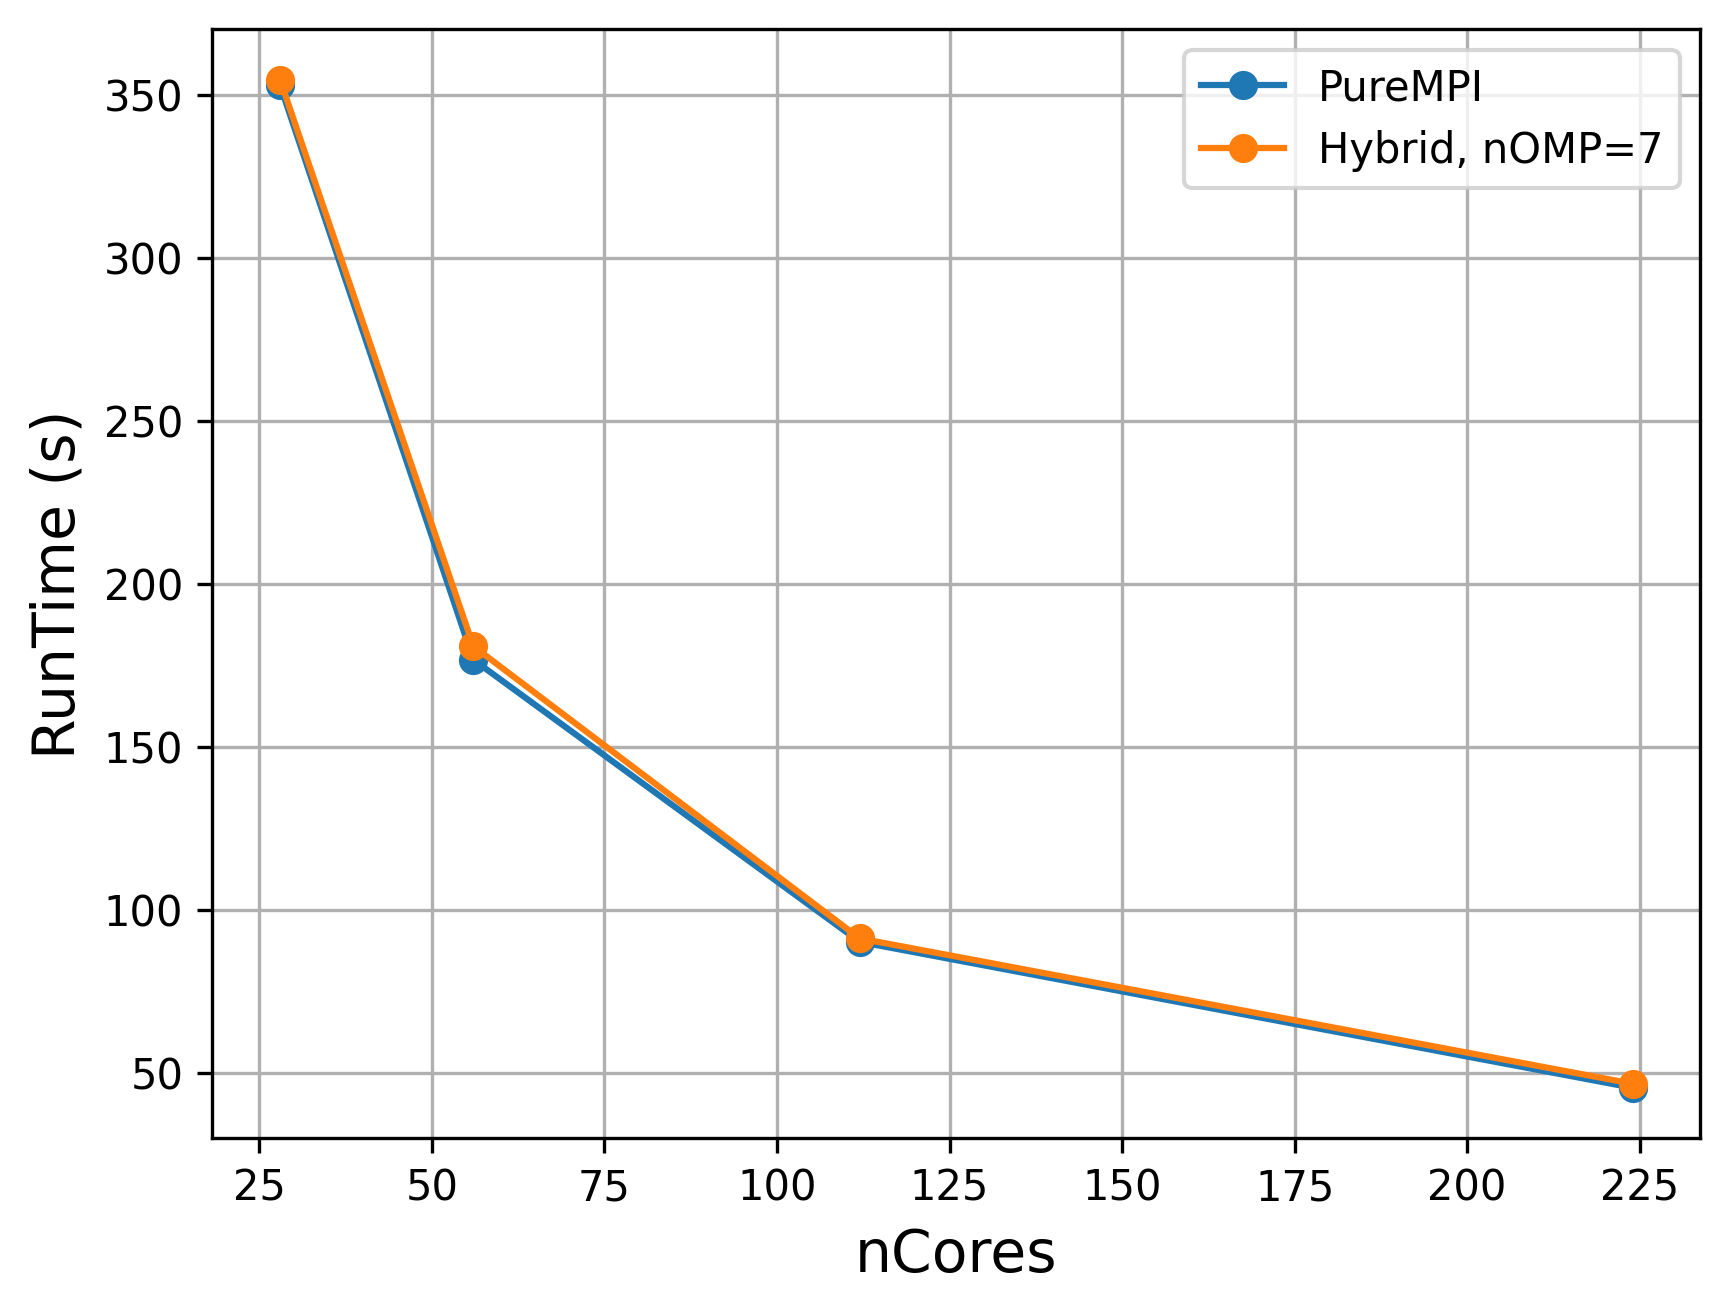
\includegraphics[width=.75\textwidth,keepaspectratio=true]{../figs/3_hybrid_vs_mpi.png}
	\caption{Performance Comparison between PureMPI and Hybrid Implementation}
	\label{fig:compare_hybrid}
\end{figure}
\subsection{Profiling Hyrbid CG}
With a first glance at the Figure \ref{fig:hybrid_scalasca1}, we can see that the structure of the hybrid profiling is quite different to what we had for pure MPI jobs. Besides the time spent for Computation and MPI, there are also time for OpenMP and for Idle threads. In computation, we can see that there is a big imbalance workload between master threads and child threads. For example, in the 0th rank, the master threads works for 61 seconds while its child threads only work for roughly 42 seconds. 

\begin{figure}[htpb]
	\centering
	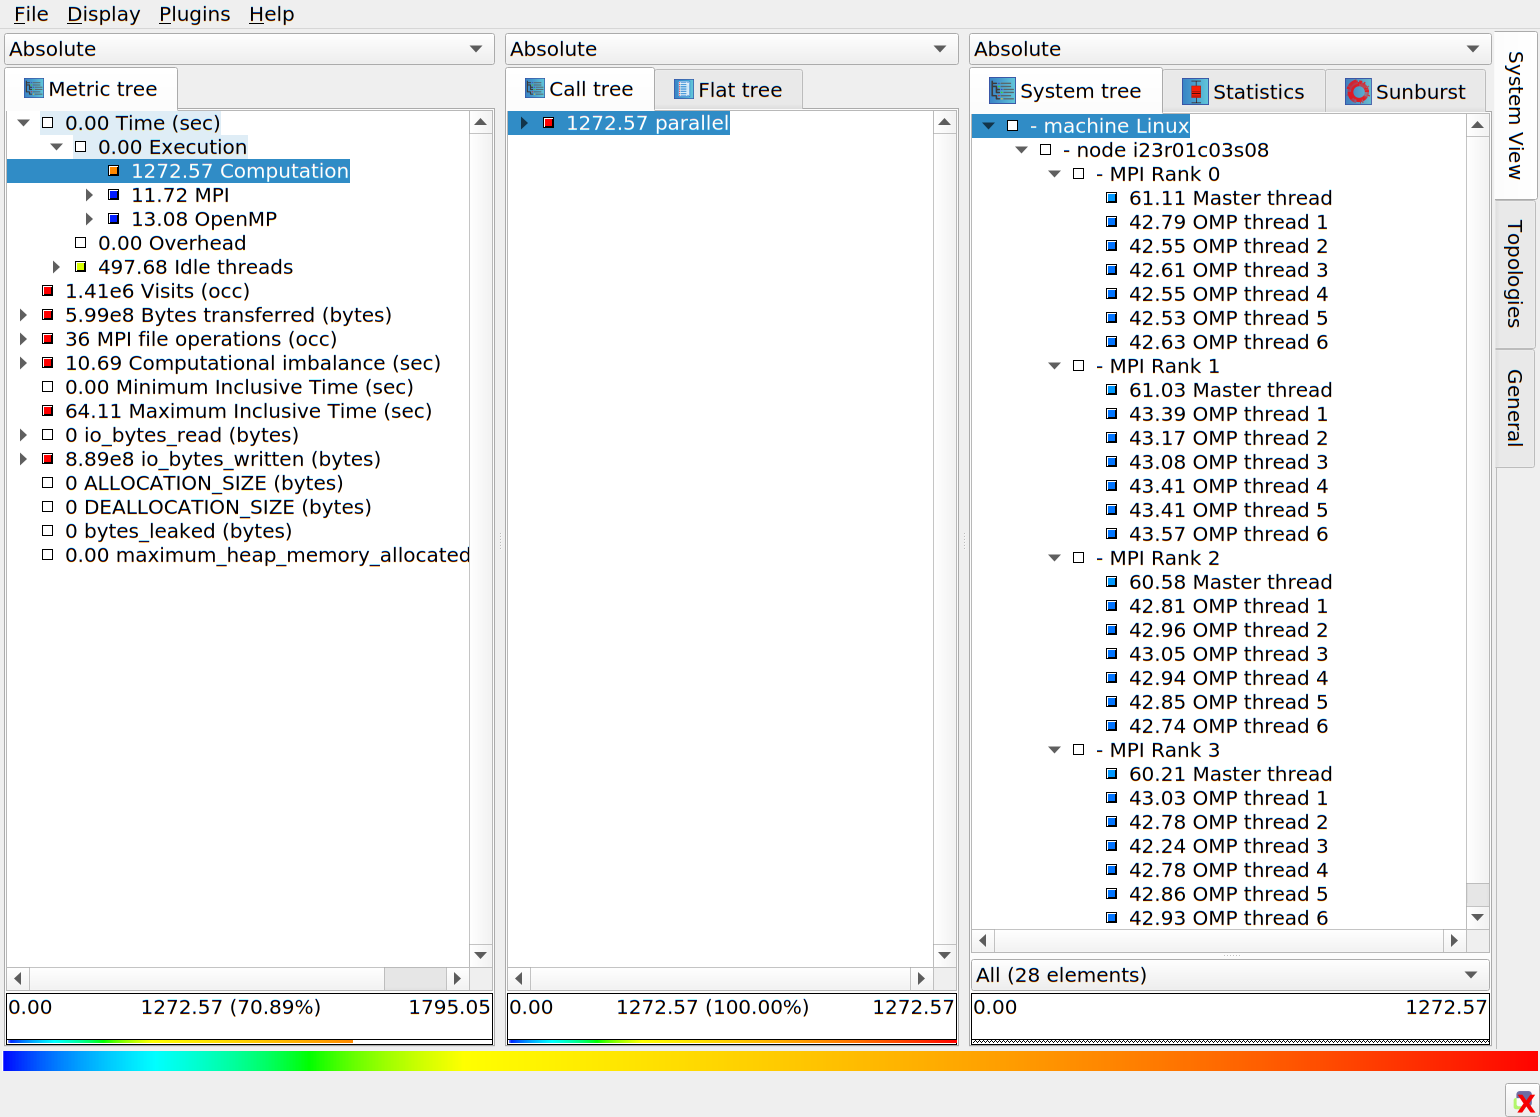
\includegraphics[width=.9\textwidth,keepaspectratio=true]{../figs/3_3_hybrid_computation.png}
	\caption{Manual Profiling of \textit{solve()}, Computation Workload}
	\label{fig:hybrid_scalasca1}
\end{figure}

At first we thought that this is a problem from load balance. But after have a look in more detail which is presented in the Figure \ref{fig:hybrid_scalasca2}, we see that in each \textit{!\$omp parallel} region, for example the one at \textit{@general.cpp:254} (which is inside of \textit{g\_scale\_add}), all threads have pretty equal work load and spent roughly the same time inside each function. It means the difference in runtime of master threads and child threads we observed before is due to the fact that the master threads are also the threads which handle the MPI calls, while other child threads - who only do work in parallel region - need to wait/be idle. 

\begin{figure}[htpb]
	\centering
	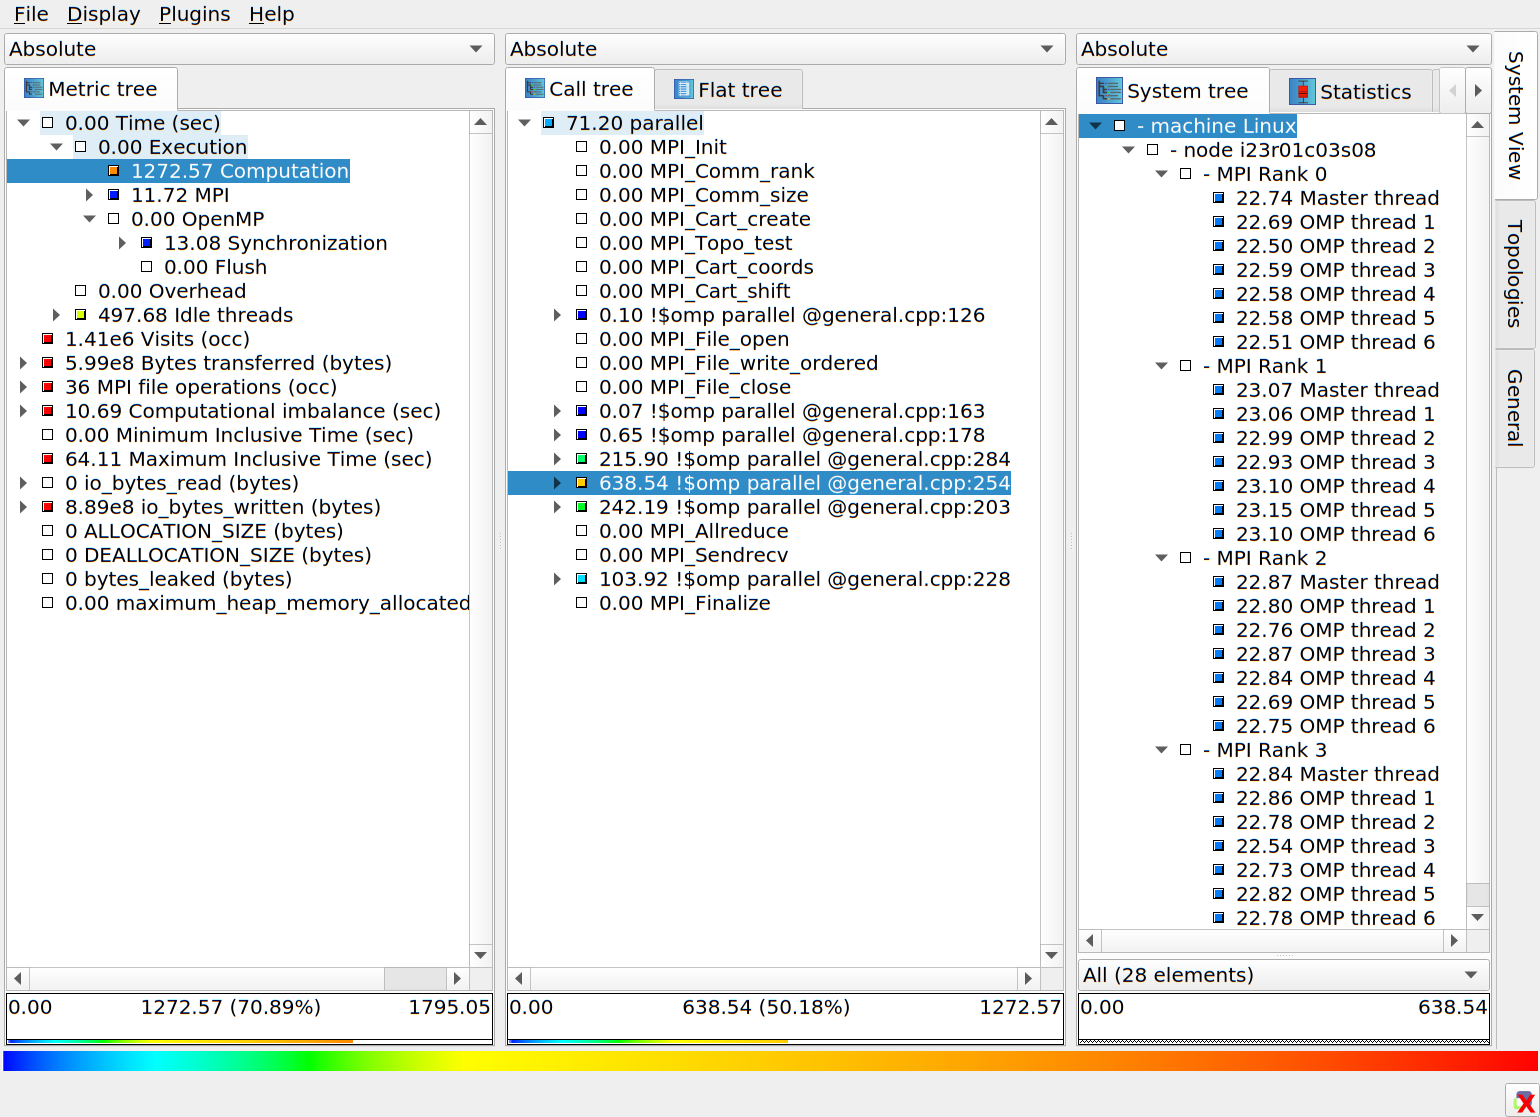
\includegraphics[width=.9\textwidth,keepaspectratio=true]{../figs/3_3_hybrid_openmp_loadbalance.png}
	\caption{Manual Profiling of \textit{solve()}, OpenMP Thread Load Balance}
	\label{fig:hybrid_scalasca2}
\end{figure}

This can be proved by the Figure \ref{fig:hybrid_scalasca3}, where we can see that the idle time of child threads are all during the MPI calls.
\begin{figure}[htpb]
	\centering
	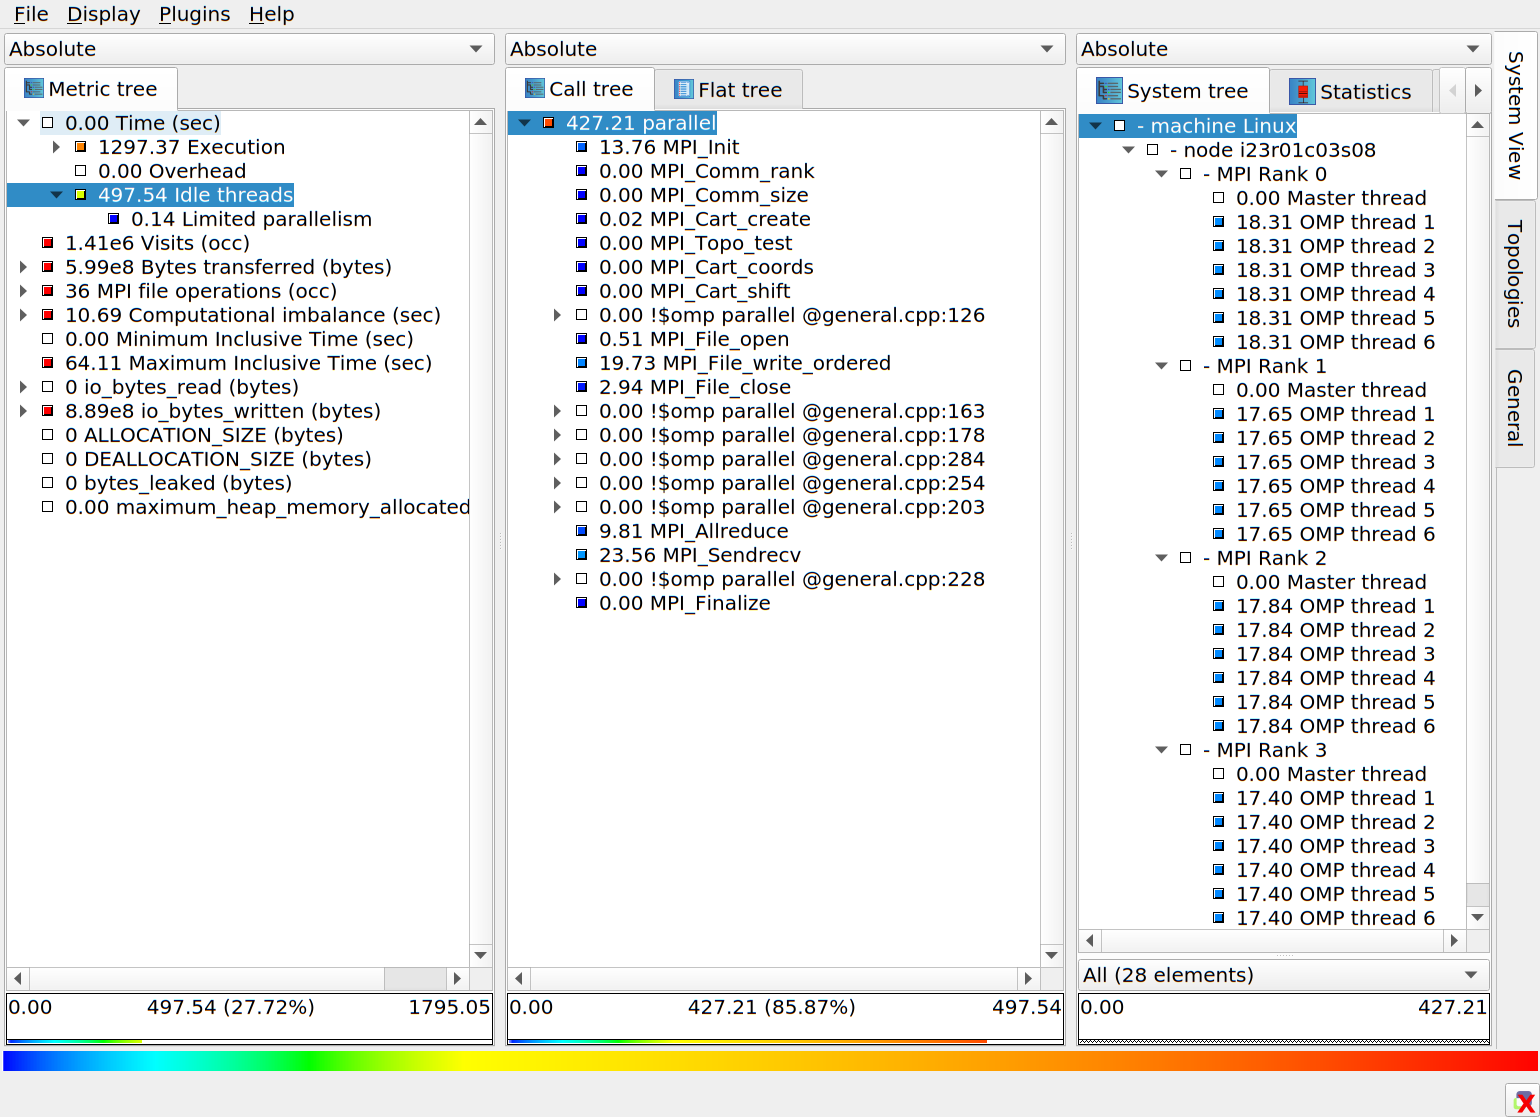
\includegraphics[width=.9\textwidth,keepaspectratio=true]{../figs/3_3_hybrid_idle.png}
	\caption{Manual Profiling of \textit{solve()}, Thread Idle}
	\label{fig:hybrid_scalasca3}
\end{figure}
\subsection{Discussion}
The Scalasca tool is very handful and simple to use, even with the Hybrid program. In our case, however, since all OpenMP load balance is pretty good and there is a very small portion of Computational Imbalance, we could not come up with any further possible optimisations based on this profile outputs, even though we expected hybrid would have a better performance then purely MPI but it did not happen.

\section{Likwid-perfctr (3P)}
1.a)
\begin{lstlisting}[frame=single]
#ifdef LIKWID_PERFMON
#include <likwid-marker.h>
#else
#define LIKWID_MARKER_INIT
#define LIKWID_MARKER_THREADINIT
#define LIKWID_MARKER_SWITCH
#define LIKWID_MARKER_REGISTER(regionTag)
#define LIKWID_MARKER_START(regionTag)
#define LIKWID_MARKER_STOP(regionTag)
#define LIKWID_MARKER_CLOSE
#define LIKWID_MARKER_GET(regionTag, nevents, events, time, count)
#endif

void gravity(double dt, RigidBody* bodies, int T) {
  LIKWID_MARKER_START("gravity");
  for (int t = 0; t < T; ++t) {
    bodies->move(0.0, 0.0, 0.5 * 9.81 * dt * dt);
  }
  LIKWID_MARKER_STOP("gravity");
}

int main() {
    LIKWID_MARKER_INIT; 
    ...
    LIKWID_MARKER_CLOSE;
    return 0;
}
\end{lstlisting}
The following command can be used to compile the code with LIKWID with gcc
\begin{lstlisting}[frame=single]
    $ gcc -DLIKWID_PERFMON -L$LIKWID_LIB -llikwid -I$LIKWID_INCLUDE 
    <SRC> -o <EXEC> 
\end{lstlisting}

LIKWID\_LIB and LIKWID\_INCLUDE will be automatically set when we load LIKWID in our server(module load likwid).\\
To run the application, using the following command
\begin{lstlisting}[frame=single]
    $ likwid-perfctr -C process_ids -g event -m <EXEC> 
\end{lstlisting}
b)
\begin{itemize}
    \item FALSE\_SHARE, not relevant since our application run with single core.
    \item TLB\_INSTR  L1 Instruction TLB miss rate/ratio, not relevant because our application is small.
    \item CACHES  Cache bandwidth in MBytes/s, relevan to have a overview of cashes's information since our application is data hard related.
    \item UOPS\_EXEC  UOPs execution, not relevant since we don't have much branch in our code.
    \item UOPS\_RETIRE  UOPs retirement, not relevant, same as above.
    \item BRANCH  Branch prediction miss rate/ratio, not relevant since no branch in our app.
    \item FLOPS\_AVX  Packed AVX MFLOP/s, not relevant, didn't use much FLOP in our app.
    \item L2CACHE  L2 cache miss rate/ratio, relevant, to see if bodies is still in cache.
    \item L3  L3 cache bandwidth in MBytes/s, not quite relevant since L3 is the last layer and our app is small. L3<->main memory is not so important for us.
    \item QPI  QPI Link Layer data, not relevant, we didn't use the network.
    \item UOPS  UOPs execution info, not relevant, same reason as in UOPS\_EXEC.
    \item NUMA  Local and remote memory accesses, not relevant, no remote memory used.
    \item ENERGY  Power and Energy consumption, not relevant. our purpose is not energy saving.
    \item L3CACHE  L3 cache miss rate/ratio, as the last layer, L3 may not be so relevant. same reason as above
    \item ICACHE  Instruction cache miss rate/ratio, not relevant app is small.
    \item CBOX  CBOX related data and metrics, may be relevant, but most likely not since our app is too small to use the last layer.
    \item CYCLE\_ACTIVITY  Cycle Activities, not relevant
    \item TLB\_DATA  L2 data TLB miss rate/ratio, relevant since our app is data hard related.
    \item MEM  Main memory bandwidth in MBytes/s, not relevant, (result all 0?
    \item DATA  Load to store ratio, relevant, help us to find out if store is the bottleneck or load.
    \item L2  L2 cache bandwidth in MBytes/s, relevant to see how many data is loaded and evicted.
    \item DIVIDE  Divide unit information, not relevant since no divide in app.
    \item CYCLE\_STALLS  Cycle Activities (Stalls), useful for us to find out the bottleneck.
    \item CLOCK  Power and Energy consumption, not relevant. our app is too small to measure the energy consumption.
\end{itemize}
c)
\begin{lstlisting}
+----------------------+------------+
|        Metric        | HWThread 0 |
+----------------------+------------+
|  Runtime (RDTSC) [s] |     0.0024 |
| Runtime unhalted [s] |     0.0027 |
|      Clock [MHz]     |  2899.6409 |
|          CPI         |    13.4467 |
|    L2 request rate   |     1.4124 |
|     L2 miss rate     |     0.4627 |
|     L2 miss ratio    |     0.3276 |
+----------------------+------------+
\end{lstlisting}

We found that the cache miss rate of L2 is quite high because everytime we call the function, the rigidbody needs to be reloaded. Our idea is, instead of update all rigidbody together once in gravity, we can rewrite the gravity function so that it only update one rigidbody for a given time period.\\
\begin{lstlisting}
void gravity(double dt, RigidBody* bodies, int T) {
    for (int t = 0; t < T; ++t) {
      bodies->move(0.0, 0.0, 0.5 * 9.81 * dt * dt);
    }
  }
int main() {
    ...
    for (int n = 0; n < N; ++n) {
        gravity(0.001, bodies[n], T);
    }
    ...
}
\end{lstlisting}
With this, we incresed the Bandwidth from 341.077062 to 1529.414464 and reduced the L2 miss rate from 0.4627 to 0.0042.

2.a) Assume we use 4 threads for our application, then the task distributed to each core is :
\begin{align*}
    core 0&: \quad (N+(N-1)+...+N-N/4 +1)=9381250 FLOPS\\
    core1&: \quad (N-N/4)+...+(N-N/2+1)=6255000FLOPS\\
    core 2&:  \quad (N-N/2)+...+(N-3*N/4+1) = 3131250FLOPS\\
    core 3&: \quad (N-3*N/4+1) + ... +1 = 3750FLOPS
\end{align*}

From the results we can easily see that there's a big gap of flops between different threads. The reason is that the task is upper-triangular matrix times vector multipli- cation. 
The default schedule of $\#pragma omp for$ is static, which means omp simply divide the task by rows with $rows/OMP\_NUM\_THREADS$. But the calculation for each row is different, the upper the row is, the more calculation it needs to be done.
That is the reason why there's a load imbalance.\\
b)
\begin{lstlisting}
+-----------------------+---------+------------+------------+
|         Event         | Counter | HWThread 0 | HWThread 1 |
+-----------------------+---------+------------+------------+
|     AVX_INSTS_CALC    |   PMC0  |  174701500 |  108035300 |
+-----------------------+---------+------------+------------+

+-----------------------+---------+------------+------------+------------+
|         Event         | Counter | HWThread 0 | HWThread 1 | HWThread 2 | 
|     AVX_INSTS_CALC    |   PMC0  |  165725700 |  283130100 |  170502800 |   
+-----------------------+---------+------------+------------+------------+
                                  +------------+  
                                  | HWThread 3 |
                                  | 57890290   |
                                  +------------+
\end{lstlisting}
By running the application with FLOPS\_AVX for different numbers of threads, we can see from the metrics AVX\_INSTS\_CALC that the task distributed
to different core is quite different which means we have found a load balance here. But this metrics can not always find the load imbalance for us. Reason see in sub task d.\\
\\
c) Since our application do not have much branches and thus there's no need to predict branch. So there won't be too much overhead spent on executing wrong instructions,
which means INSTR\_RETIRED\_ANY can in some sense represent the work load for each task.\\
\\
d)To solve this problem, the easiest way is using dynamic schedule of omp. We tried with $schedule(dynamic, 10)$ with 4 threads, and get the result as follows:
\begin{lstlisting}
    +-----------------------+---------+------------+------------+------------                                
    |         Event         | Counter | HWThread 0 | HWThread 1 | HWThread 2 
    +-----------------------+---------+------------+------------+------------
    |   INSTR_RETIRED_ANY   |  FIXC0  |  587691000 |  665369900 |  719993700 
    |     AVX_INSTS_CALC    |   PMC0  |  105834700 |  243815400 |  269732900 
    +-----------------------+---------+------------+------------+------------
                                      +------------+
                                      | HWThread 3 |
                                      +------------+
                                      |  710925800 |
                                      |  272558700 |
                                      +------------+ 
\end{lstlisting}
We can see now the flops of thread 1,2,3 are quite similar but not thread 0. But take a look at INSTR\_RETIRED\_ANY,
we realize that the reason why thread 0 didn't do as much flops as other threads is that thread 0 is the master thread and need to also be responsible for scheduling stuff.
So we can not say that there's a load imbalance here because the total instructions each core have done here is almost the same.
In this case, Not only can't AVX\_INSTS\_CALC help us to find the load imbalance, it can even be misleading.

\section{Reverse Engineering with Tracing (2P)}

\subsection{Description of tracing using Intel Trace Analyzer and Collector}
Tracing is an application gives insights into the applications behavior by collecting timing information 
regarding  function calls or expliclity identified code paths.
This is generally done by calling two timestams: One before entering a function and one after exiting said function.
The differences of these timestams are then collected and mapped to the applications call paths.
In parallel applications, the respective times have also be mapped to process ids and threads, if applicable.

Intel Trace Analyzer and Collector provides the APIs, command line tools, as well as GUI-applications to first collect and later analyze and visualize these traces using the intel tools.

\paragraph{Usage of ITAC on CoolMUC2}
To use ITAC on CoolMUC2 the following commands have to be entered:
\begin{verbatim}
module unload intel-mpi intel-mkl intel
module load intel-parallel-studio/2018
#everything is now in $INTEL_PARALLEL_STUDIO_BASE
. $INTEL_PARALLEL_STUDIO_BASE/bin/compilervars.sh intel64
. $INTEL_PARALLEL_STUDIO_BASE/vtune_amplifier/amplxe-vars.sh
. $INTEL_PARALLEL_STUDIO_BASE/itac_latest/bin/itacvars.sh
. $INTEL_PARALLEL_STUDIO_BASE_impi/2018.4.274/bin64/mpivars.sh
\end{verbatim}
This makes the itac, vtune and compiler tools available.

\paragraph{Instrumentation using ITAC by commandline}

To compile for tracing, the \textit{-trace} flag has to be set for the intel compiler.
\begin{verbatim}
mpiicc -trace cool_mpi_app.c -I$INTEL_PARALLEL_STUDIO_BASE/itac_latest/include
\end{verbatim}

By giving command line arguments, such as \textit{tcollect} all functions can be instrumented for collection automatically.
\begin{verbatim}
mpiicc -tcollect -trace cool_mpi_app.c \
-I$INTEL_PARALLEL_STUDIO_BASE/itac_latest/include
\end{verbatim}

Additionally specific functions can be selected given by specifing the functions to be collected in a ``filter file'', in case not all functions are desired for collection.
This is done by naming them in a file the filter file.
E.g.\ for the the \textit{cool\_mpi\_app.c}, a filter file \textit{filterfile.flt} may look like:
\begin{verbatim}
do_something on
\end{verbatim}
Where valid parameters for the functions are \textit{on} of \textit{off}.
The specific functions are then automatically instrumented if set to on.
\begin{verbatim}
mpiicc -tcollect-filter filterfile.flt -trace cool_mpi_app.c \
	-I$INTEL_PARALLEL_STUDIO_BASE/itac_latest/include
\end{verbatim}

\paragraph{Instrumentation Using ITAC by API}
Alternatively event handler can be introduced by hand. 
(The example shown in the following is the as of \textit{superusefulITAC.cpp}, where the manual tracing using the \textit{Stopwatch.h} functonality is replaced by \textit{VT} calls as describied in the \textit{ITAC} documentation.)
This is done by defining a VT function:
\begin{verbatim}
static int _myregid
char *name="My region ID";
ierr=VT_funcdef(name, VT_NOCLASS, &_myregid);
assert(ierr == VT_OK);
\end{verbatim}
This \textit{\_myregionid} handle can now be used to identify specific regions within the code using the functions
\textit{VT\_begin(\_myregionid)} and \textit{VT\_end(\_myregionid)}. 
This is especially usefull when a region is not soley defined by a function or shall spann multiple functions. E.g.:
\begin{verbatim}
\\ Some work
VT_begin(_myregionid_handle)
for(int=0;i<5;i++){
function1();
function2();
function3();
}
VT_end(_myregionid_handle)
\\ Some further work
\end{verbatim}

\subsection{Parameter Analysis of \textit{cool\_mpi\_app.exe}}

In this task, we ran the \textit{cool\_mpi\_app.exe} with 2 MPI processes. We tested different parameters and their influences to the total runtime, ratio between the time spent for the 'computation' and MPI rountines, and waiting time at the bariers. \\
From the Figure \ref{fig:trace1} to \ref{fig:trace2}, we can see that when double the fourth parameter, we got the total runtime increase by 2, in which the time for application in the Rank 0 and the time for MPI in Rank 1 kept almost the same, but the time for MPI in rank 0 and the time for application in Rank are doubled, leading to the time for Rank 0 to wait at the barrier also doubled. \\
From the Figure \ref{fig:trace1} to \ref{fig:trace3}, we can see that when double the third parameter, we got the total runtime increase by 1.5. We noticed that the time for Application in both Ranks increased by 2 times in the \ref{fig:trace3} in comparison to in \ref{fig:trace1}, while the time for MPI moved toward to become equal. In this test, even though the computation load is not balanced between the two ranks, we have least waiting time at the barrier, only 0.3\%. \\
From the Figure \ref{fig:trace1} to \ref{fig:trace4}, we can see that when double the second parameter, we got the total runtime increase by 2, in which the times in rank 0 increased by roughly 1.5, while for rank 1 the time for computation increases by 2 at the same time keeping constant time for MPI. The time spent at barrier for rank 0 increased roughly 25\%. \\
The last parameter-set result in \ref{fig:trace5} has similar effect as in \ref{fig:trace4}.

\begin{figure}[htpb]
	\centering
	\begin{subfigure}{0.9\textwidth}
		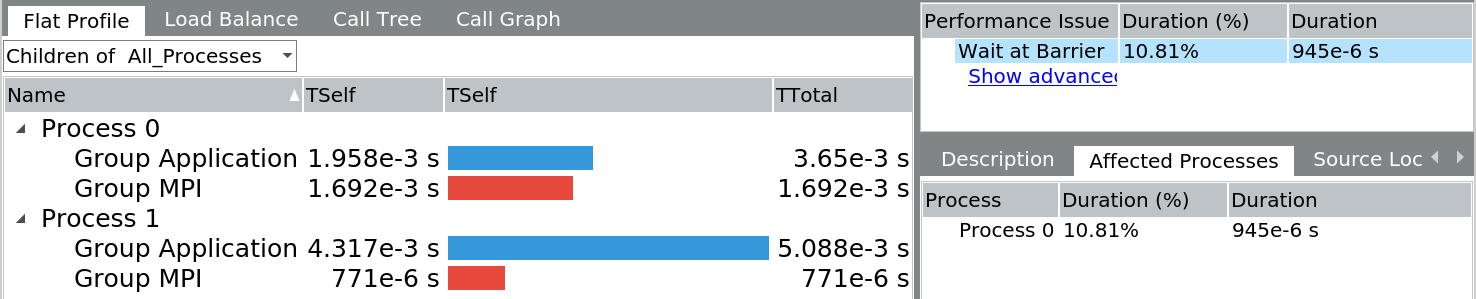
\includegraphics[width=\textwidth,keepaspectratio=true]{../figs/4_2_para_1_1_1_1.png}
		\caption{Parameters=(1 1 1 1), Total runtime = 0.00874s}
		\label{fig:trace1}
	\end{subfigure}
~ 
	\begin{subfigure}{0.9\textwidth}
	\centering
	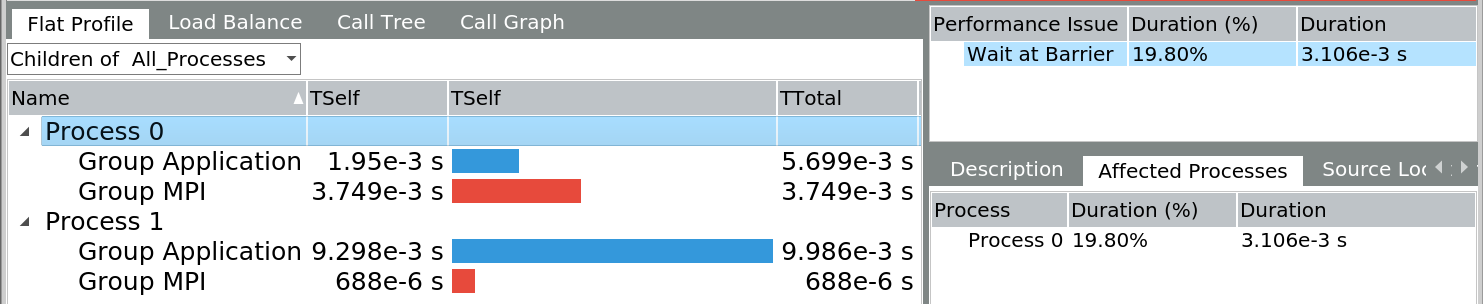
\includegraphics[width=\textwidth,keepaspectratio=true]{../figs/4_2_para_1_1_1_2.png}
	\caption{Parameters=(1 1 1 2), Total runtime = 0.0157}
	\label{fig:trace2}
	\end{subfigure}
~
	\begin{subfigure}{0.9\textwidth}
	\centering
	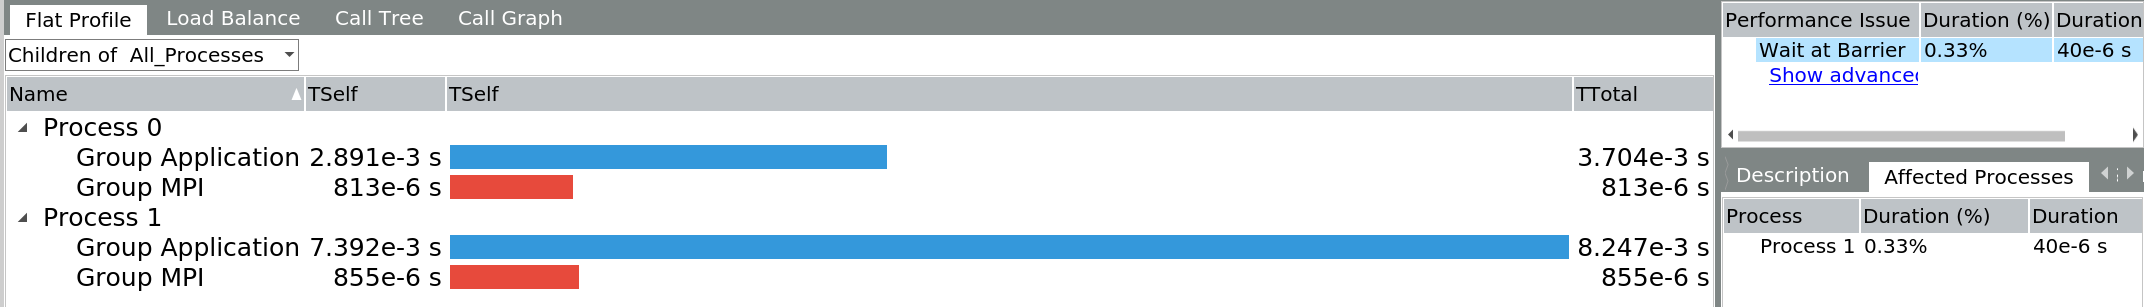
\includegraphics[width=\textwidth,keepaspectratio=true]{../figs/4_2_para_1_1_2_1.png}
	\caption{Parameters=(1 1 2 1), Total runtime = 0.012}
	\label{fig:trace3}
	\end{subfigure}
~
	\begin{subfigure}{0.9\textwidth}
	\centering
	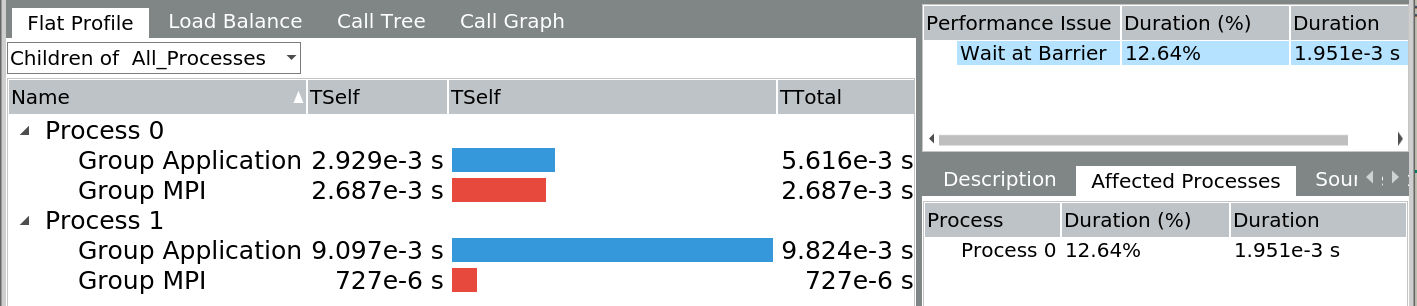
\includegraphics[width=\textwidth,keepaspectratio=true]{../figs/4_2_para_1_2_1_1.png}
	\caption{Parameters=(1 2 1 1), Total runtime = 0.0154}
	\label{fig:trace4}
	\end{subfigure}
~
	\begin{subfigure}{0.9\textwidth}
	\centering
	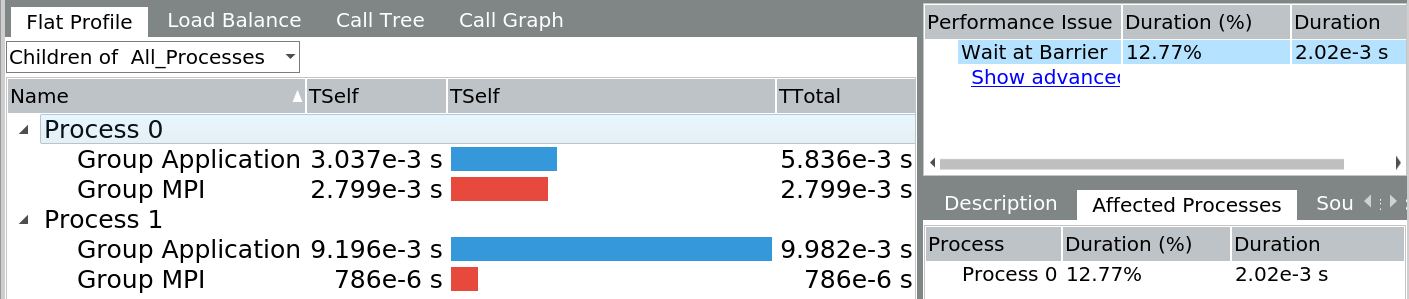
\includegraphics[width=\textwidth,keepaspectratio=true]{../figs/4_2_para_2_1_1_1.png}
	\caption{Parameters=(2 1 1 1), Total runtime = 0.0158}
	\label{fig:trace5}
	\end{subfigure}
	\caption{Trace Analyzer of \textit{cool\_mpi\_app.exe} with various parameters}
	\label{figs:trace_4.2}
\end{figure}

Besides, from the Trace analyzer, we also knew that in the black box binary, there is only \textit{MPI\_Allreduce} is used for communication. (Figure \ref{fig:trace_4.3})).
\begin{figure}[htpb]
	\centering
	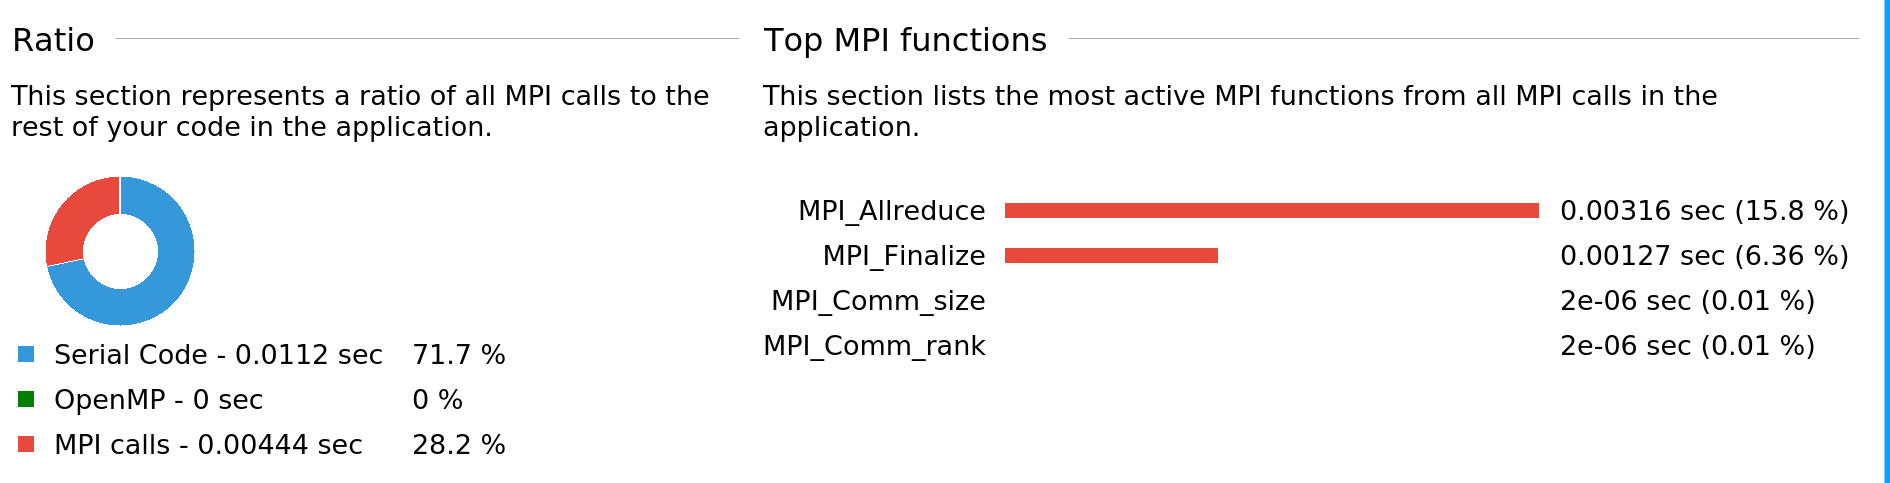
\includegraphics[width=.9\textwidth,keepaspectratio=true]{../figs/4_2_MPI_Functions.png}
	\caption{Trace Analyzer of \textit{cool\_mpi\_app.exe} - MPI Functions}
	\label{fig:trace_4.3}
\end{figure}

\subsection{Analysis of expert user's parameters}
In this taks we have parameters given by an expert: They suggest $a=10$, $b=100$, and $c_1=14$,$c_2=14$, $c_3=14$, $c_4=14$.
We run the experiment as suggested by the expert and present these in Figure~\ref{fig:expert1}.
\begin{figure}[htpb]
	\centering
	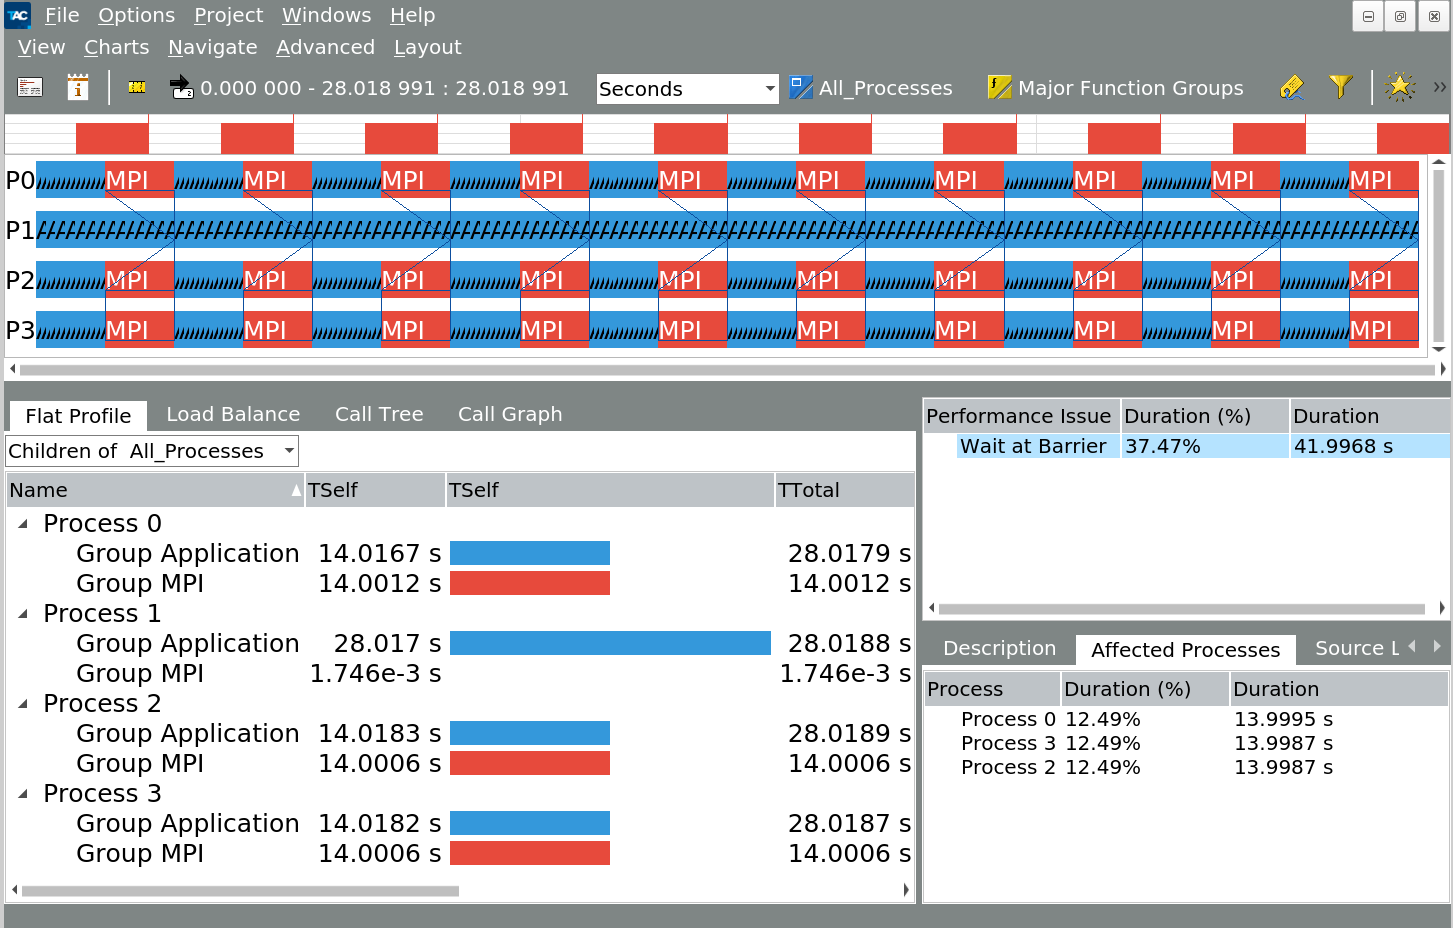
\includegraphics[width=.9\textwidth,keepaspectratio=true]{../figs/4_3_14_14_14_14.png}
	\caption{Trace Analyzer of \textit{Expert parameters} - 14 14 14 14}
	\label{fig:expert1}
\end{figure}
Figure~\ref{fig:expert1} shows a total execution time of 28 seconds. The trace shows that ranks 0, 2 and 3 have substantial waiting times of 14 seconds. Rank 1 has no waiting time and their workload is double the workload of 0, 2 and 3.
Therefore, we suggest an improved parameterset: The parameters 10 and 100 for $a$ and $b$ are fixed, similarly $c_1+c_2+c_3+c_4 \overset{!}{=} 56$ is required. Therefore we suggest to half the time of rank 1 while minimizing the other parameters. Since $14/2=7$, but $(56-7)/3$ is not integer, we suggest $c_2=8$. This results in the parameters $c_1=16$, $c_2=8$, $c_3=16$, $c_3=16$, resulting in balanced parameters for ranks 0,2 and 3.
We run this parameterset and evaluated as seen in Figure~\ref{fig:expert2}.
\begin{figure}[htpb]
	\centering
	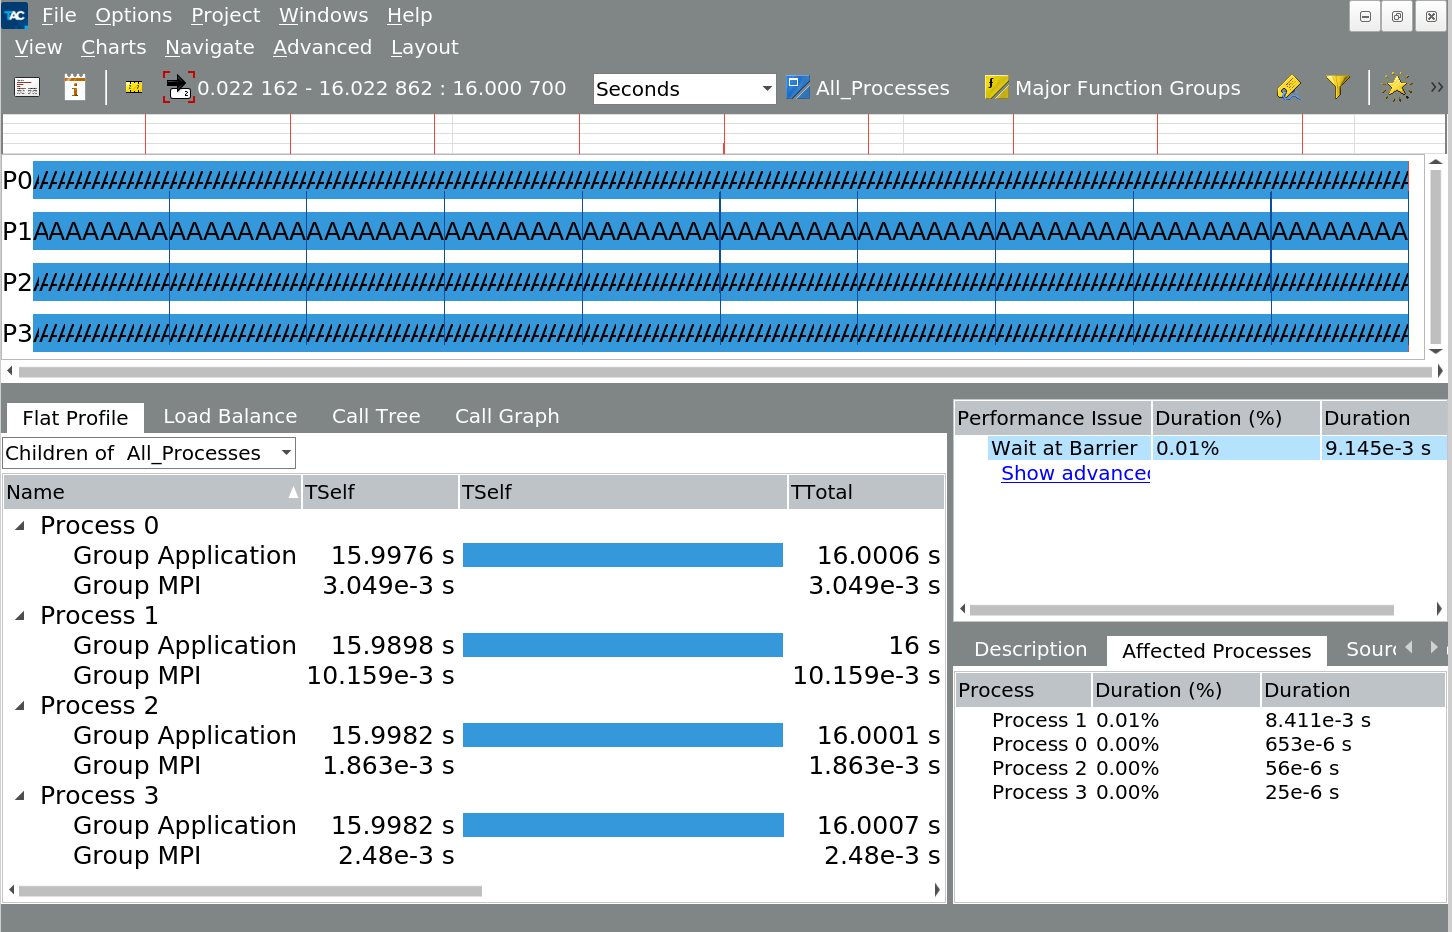
\includegraphics[width=.9\textwidth,keepaspectratio=true]{../figs/4_3_16_8_16_16.png}
	\caption{Trace Analyzer of optimal parameters - 16 8 16 16}
	\label{fig:expert2}
\end{figure}
Figure~\ref{fig:expert2} shows a total execution time of 16 seconds. This is a speedup of $1.75$. 
The processes show no waiting time and for parameters a=10 and b=100 this appears to be an optimal input parameter set from an MPI perspective.
To verify this, an evaluation of reducing the paramter of $c_2$ further to $c_2=7$ is evaluated (Fig.~\ref{fig:expert3a}).
Additionally it is evaluated if the parameter doesn't need that much reduction by setting it to $c_2=9$ (Fig.~\ref{fig:expert3b}).

\begin{figure}[htpb]
	\centering
    \begin{subfigure}{\textwidth}
	\centering
	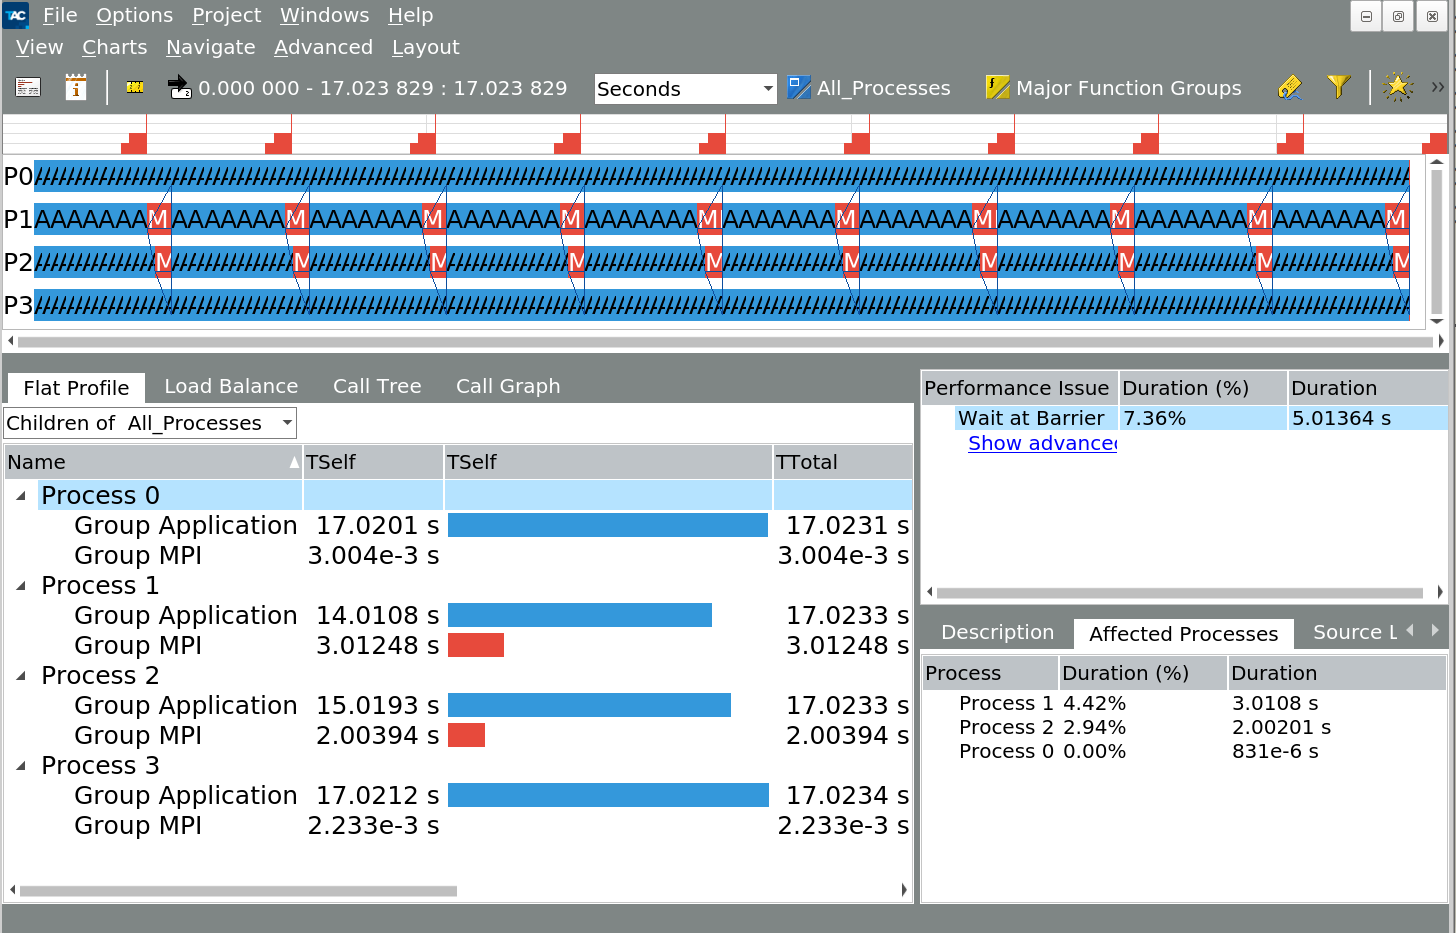
\includegraphics[width=.9\textwidth,keepaspectratio=true]{../figs/4_3_17_7_15_17.png}
	\caption{Trace of parameters 17 7 15 17}
	\label{fig:expert3a}
    \end{subfigure}
~\newline
~\newline
    \begin{subfigure}{\textwidth}
	\centering
	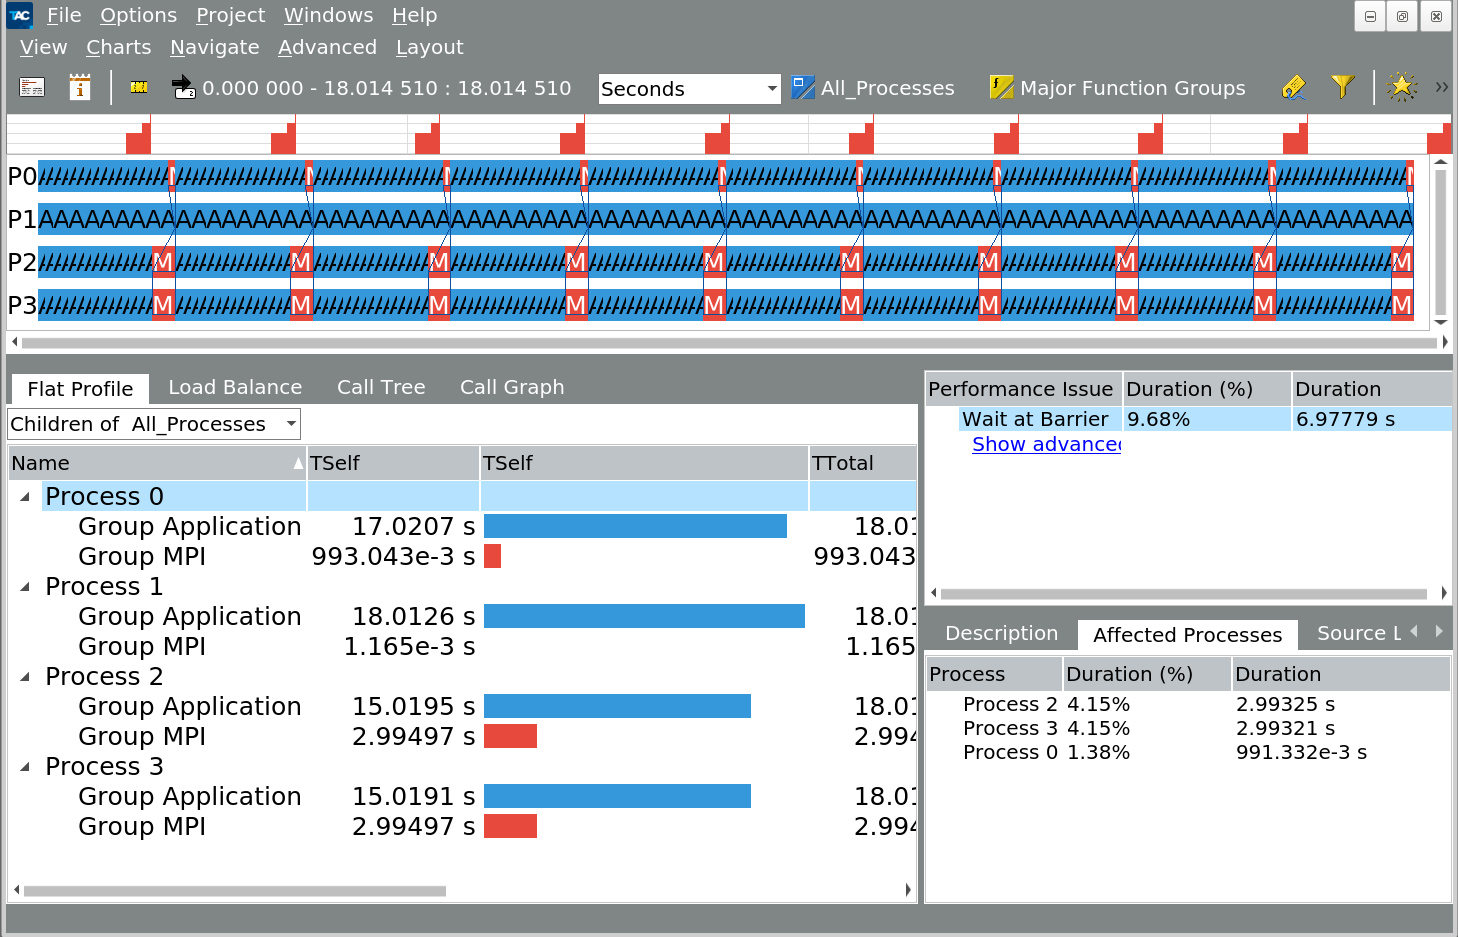
\includegraphics[width=.9\textwidth,keepaspectratio=true]{../figs/4_3_17_9_15_15.png}
	\caption{Trace of parameters 17 9 15 15}
	\label{fig:expert3b}
    \end{subfigure}
	\caption{Trace Analyzer of additional parameters -- non-optimal} 
    \label{fig:expert3}
\end{figure}
Figure~\ref{fig:expert3a} shows that the paramters $c_2=7$ would improve the execution time, however due to the restriction of $c_1+c_2+c_3+c_4 \overset{!}{=} 56 $ the processes with parameter 17 are now the bottleneck. 
These ranks are busy, but their parameters can no be reduced further as the sum has to be 56, and at least one of them will increase when trying to reduce the remaining parameters. This inhibits to load balance this parameter suggestion further, which makes $c_2<8$ not practical.

Figure~\ref{fig:expert3b} inquires if the parameters $c_2$ could be increased and wether the paramter $c_2=8$ is choosen too small. By setting the parameter $c_2=9$ and choosing the other parameters accordingly ($c_1=17$, $c_3=15$, $c_4=15$), we can see that now rank 1 is busy while the other ranks are waiting for it. Therefore $c_2$ should be reduced furhter.
With the considerations from both Figure~\ref{fig:expert3a} and ~\ref{fig:expert3b} we see that the parameters from Figure~\ref{fig:expert2} are already optimal.


\medskip
%\printbibliography
\bibliography{myref}{}
\bibliographystyle{plain}

\end{document}


